\ifx\ucebnice\undefined
\documentclass[a4paper,10pt,oneside]{article}
\usepackage{latexsym}
\usepackage{amsmath}
\usepackage{amsfonts}
\usepackage{amsthm}
\usepackage{amssymb}
\usepackage{fncylab}
\usepackage{comment}
\usepackage{float}
\usepackage{wrapfig}
\usepackage{tikz}
\usepackage{tikz-qtree}
\usepackage{url}
\usepackage[bookmarks, colorlinks=false, 
            pdftitle={Úvod do programování --- Algoritmy},
            pdfauthor={Jonathan L. Verner}, 
            pdfsubject={Algoritmy a složitost}, 
            pdfkeywords={algoritmus, složitost, Python, třídění, grafy},
            bookmarksdepth=3
            ]{hyperref}
\usepackage[margin=1cm]{geometry}
\usetikzlibrary{decorations.fractals,chains,fit,shapes,patterns}
\usepackage[utf8]{inputenc}
\usepackage[T1]{fontenc}
\usepackage{attachfile}
\relpenalty=9999
\binoppenalty=9999


%----------definitions---------------------------


%math definitions

\newcommand{\R}{\mathbb R}
\newcommand{\C}{{\mathcal C}}
\newcommand{\F}{{{\mathcal F}}}
\newcommand{\U}{{{\mathcal U}}}
\newcommand{\V}{{{\mathcal V}}}
\newcommand{\cont}{{\mathfrak{c}}}
\newcommand{\force}{\Vdash}
\newcommand{\pw}{{{\mathcal P}}}
\newcommand{\MU}{{\mathbb{M}_{\mathcal{U}}}}
\newcommand{\pomega}{\pw(\omega)}


\newcommand{\src}[3]{%
\begin{program}%
\caption{#2\hfill%
\attachfile[author={Jonathan Verner},
            description={Source code for #2},
            mimetype={text/x-python},
            print=false,
            icon={Paperclip}]{kod/#1}}
\label{#3}\includecode[Python]{kod/#1}
\end{program}}


%---------numbering of the theorems------------
 \swapnumbers

 \newtheorem*{theorem*}{Theorem}
 \newtheorem{theorem}[subsection]{Theorem}
 \newtheorem{proposition}[subsection]{Proposition}
 \newtheorem{observation}[subsection]{Observation}
 \newtheorem{fact}[subsection]{Fact}
 \newtheorem{lemma}[subsection]{Lemma}
 \theoremstyle{definition}
 \newtheorem{definition}[subsection]{Definice}
 \newtheorem{question}[subsection]{Problém}
 \newtheorem{ukol}{Úloha}
 \newtheorem{cviceni}[subsection]{Cvičení}
 \newtheorem{cviceniH}[subsection]{Cvičení (*)}
 \newtheorem*{reseniIMPL*}{Řešení}
 \specialcomment{reseni}{\begin{reseniIMPL*}}{\end{reseniIMPL*}}
 \excludecomment{reseni}
 \excludecomment{todo}
 \newtheorem*{comments*}{Komentáře}
 \newtheorem*{definition*}{Definice}
 \newtheorem*{question*}{Question}
 \newtheorem{notation}[subsection]{Notation}
 \newtheorem{remark}[subsection]{Poznámka}
 \newtheorem{remark*}[subsection]{Poznámka}
 \newtheorem*{note}{Poznámka}
 \newtheorem*{ack}{Acknowledgements}
 \floatstyle{ruled}
 \newfloat{program}{htbp}{listings}[section]
 \floatname{program}{Algoritmus}
 
 \hypersetup{
    colorlinks,%
    citecolor=black,%
    filecolor=black,%
    linkcolor=black,%
    urlcolor=black
}
 
\pdfinfo{
      /Author (Jonathan Verner)
      /Title (ALG110006 Úvod do programování: Poznámky k přednášce, LS)
      /Subject (programování, algoritmy)
      /Keywords (quicksort,heapsort,dijsktra,graph,euclid)
   }
\include{pythonlisting}

\lstset{
numbers=left,
stepnumber=1,
numbersep=5pt,
numberstyle=\small\color{black}
}
%-------------opening--------------------------
\begin{document}
\title{}

% \author{Jonathan Verner}
% \address{Department of Logic, Charles University\\
% Palachovo nám. 2\\ 116 38 Praha 1, Czech Republic}
% \email{jonathan.verner{@}ff.cuni.cz}
%\thanks{The author was partially supported by }

%\subjclass[2010]{Primary }
%\keywords{}

%\begin{abstract}
%\end{abstract}
%\maketitle
\thispagestyle{empty}
\pagestyle{empty}
%\hsize=16cm
\parindent=0cm
\parskip=0.2cm

\setcounter{section}{3}
\fi
\section{Analýza jazyka}
V této kapitole se podíváme na problém analýzy jazyka.  Nepůjde nám o přirozené jazyky ---
to by přesahovalo možnosti úvodního kurzu --- ale o jazyky tzv. formální. Formální jazyky
jsou jazyky, které mají přesně specifikovánu syntax, t.j. co je a co není v jazyce přípustné. 
Co to znamená \emph{přesně} specifikovat? Dohodněme se, že pro naše účely to znamená,
že je možné o daném řetězci automaticky rozhodnout, zda je v jazyce přípustný či nikoliv.

\begin{doplneni}
Přirozené jazyky tuto podmínku nesplňují, protože přípustnost je nejednoznačná ---
o přípustnosti nějaké věty se často neshodnou ani lingvisté. Jednoduchým diagonálním 
argumentem však lze ``zkonstruovat'' jazyky, kde je přípustnost daná jednoznačně, nicméně
neexistuje algoritmus, který by o přípustnosti rozhodl.  Takové jazyky nás však zajímat nebudou.
\end{doplneni}

Příkladem formálního jazyka je třeba samotný Python. Dalším příkladem může být třeba
jazyk nějaké matematické teorie.  Nebo html, jazyk ve kterém se píší webové stránky. Toto
všechno jsou relativně komplikované jazyky, kterým odpovídají i (relativně) komplikované
rozhodovací algoritmy.  My si ukážeme několik jednodušších jazyků a algoritmy, které rozhodují o 
přípustnosti pro tyto jazyky. Nejprve se však budeme zabývat jednodušším problémem ---
vyhledáváním v textu.  Optimální algoritmus pro vyhledávání nás totiž navede k definici
tzv. regulárních jazyků.

\subsection{Vyhledávání v textu}

Následující úlohu zná každý, kdo v textovém editoru někdy použil funkci ``najdi'' (find).

\begin{ukol} Nalezněte v daném textu (posloupnosti znaků) všechny výskyty nějakého slova 
(věty, posloupnosti znaků).
\end{ukol}

První řešení, které nás napadne, může vypadat třeba takto:

\srchere{dumbfind}{Naivní Vyhledávání}

Vnější cyklus postupně prochází celý text a vnitřní cyklus na každé pozici testuje, zda
se tam nevyskytuje hledaná posloupnost. Tento vnitřní test provede nejvýše \(m\) operací,
kde \(m\) je délka hledaného řetězce. Celková složitost algoritmu je tedy \(O(n\cdot m)\), 
kde \(n\) je délka textu. Na první pohled nás napadne, že lépe to snad ani nejde. 
Uvědomme si však, že algoritmus dělá spoustu zbytečné práce. Představme si, že hledáme
řetězec {\tt aaaaa} ({\tt s}) v řetězci {\tt aaaazzzz} ({\tt text}). V první iteraci zjistíme, že na pozici {\tt 0}
se řetězec nenachází, protože páté písmeno je {\tt z} a ne {\tt a}. V tu chvíli však už je
zbytečné testovat všechny pozice do pátého písmena, protože náš řetězec žádné
{\tt z} neobsahuje.  Ve skutečnosti,  když testujeme výskyt řetězce na pozici {\tt tpos}
pro {\tt tpos >= 5}, všechny znaky {\tt text[tpos],...,text[tpos+4]} jsme už viděli, takže
znalost znaku {\tt text[tpos+5]} by nám teoreticky měla stačit k rozhodnutí, zda se
{\tt s} na pozici {\tt tpos} vyskytuje. Jak tuto informaci využít? Představme si, že každá
posloupnost {\tt p} čtyř znaků má přiřazeno nějaké číslo \(n_{\tt p}\). Pak lze sestrojit
tabulku, která nám pro každý znak {\tt z}, a číslo \(n_{\tt p}\) určí, 

\begin{itemize}
 \item zda je posloupnost {\tt p+z} (posloupnost {\tt p} následovaná znakem {\tt z}) je rovná hledané posloupnosti
 \item číslo \(n_{p[1:]+z}\) posloupnosti {\tt p+z} bez prvního znaku
\end{itemize}

Pokud bychom takovou tabulku měli, bylo by vyhledávání velmi jednoduché. Algoritmus
by vypadal třeba jako na výpisu \ref{alg:smartfind} (uvažujeme jednoduchý příklad kdy
hledáme řetězec {\tt aab} v posloupnosti která sestává pouze ze znaků {\tt a} a {\tt b}).

\src[firstline=2]{smartfind}{Vyhledávání za pomoci tabulky}

Je lehké nahlédnout, že složitost je nyní lineární v délce textu, t.j. \(O(n)\). Problém je
však se sestrojením tabulky (a s její velikostí). Máme-li abecedu o \(k\) znacích
(v příkladu \ref{alg:smartfind} je \(k=2\)), a hledáme řetězec délky \(m\), pak naše tabulka
bude mít velikost \(k\cdot k^{m-1}\) a tedy její výroba bude trvat \(O(k^{m})\). 
Tím bychom vyměnili složitost \(O(n\cdot m)\) za \(O(n+k^{m})\), což není příliš výhodné.

\paragraph{Konečné automaty}

Naše tabulka je ale příliš veliká. Všimněte si například, že hodnoty odpovídající
\(n_{\tt p} = 1,2\) jsou stejné.  To napovídá, že by bylo možné ušetřit. Ukážeme, 
že tabulku lze nahradit komplikovanější strukturou, tzv. konečným automatem. 
Jeho výhoda spočívá v tom, že vhodný automat  lze vytvořit v čase \(O(m)\) 
(místo \(O(2^{m})\)). Co to je konečný automat?  Ukážeme si to nejprve na příkladě
jednoduchého konečného automatu --- zakódovaného zámku na kole. 

\begin{center}
 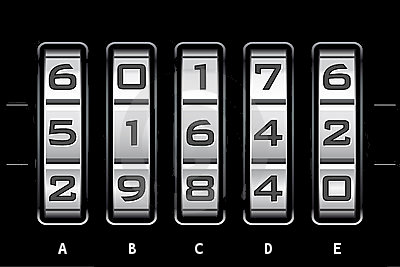
\includegraphics[width=5cm]{combination-lock}
\end{center}

Koncepčně má zámek dva stavy --- odemčeno a zamčeno.  Zadáním správného kódu 
ho člověk může ze stavu zamčeno přesunout
do stavu odemčeno.  Ve skutečnosti si však můžeme představit, že zámek má mimo
dvou základních stavů různé vnitřní stavy odpovídající různým možným kódovým
kombinacím. Jeden z těchto vnitřních stavů --- stav odpovídající správnému kódu ---
pak odpovídá globálnímu stavu odemčeno, ostatní odpovídají stavu zamčeno. 
Nastavením číslice na jednom z možných míst pak přesouváme zámek z jednoho
vnitřního stavu do jiného.

Obecná definice konečného automatu je zobecněním této konkrétní situace.

\begin{definition} \emph{Konečný automat} je dán množinou (vnitřních) stavů \(S\),
množinou vstupů (abecedou) \(\Sigma\), přechodovou funkcí \(f:S\times\Sigma\to S\)
a množinou koncových stavů \(E\subseteq S\) a jedním počátečním stavem \(s^b\in S\).
\end{definition}

V případě zámku by množina vnitřních stavů byla množina všech 5 ciferných čísel,
Množina vstupů by byla množina všech dvojic (pozice, číslice), kde pozice je jedno z 
písmen A, B, C, D, E. Přechodová funkce pak odpovídá změně stavu při zadání jedné
číslice kódu. Koncový stav je jediný --- ten který odpovídá správnému kódu. 
Počáteční stav je náhodný zamčený stav, který byl nastaven při zamykání. 

Definujme ještě co to znamená výpočet. Intuitivně je to posloupnost stavů a vstupů
začínající v počátečním stavu a končící v nějakém koncovém stavu taková, že přechod 
mezi sousedními členy této posloupnosti je dán přechodovou funkcí:

\begin{definition} \label{def:vypocet}
Posloupnost stavů \(\overline{s}=\langle s_0,\ldots, s_n\rangle\)
a vstupů \(\overline{v}=\langle v_0,\ldots, v_{n-1}\rangle\) je výpočtem automatu 
\(A=(S_A,\Sigma_A,f_A, E_A,s_A^b)\) pokud \(s_0=s_A^b\), \(s_n\in E_A\) a pro \(1\leq i\leq n-1\) 
platí \(s_{i+1} = f(s_i,v_i)\).
\end{definition}

Když se zamyslíte nad algoritmem \ref{alg:smartfind} možná Vás napadne, že by se dal
popsat jako provádění výpočtu nějakého konečného automatu. Tabulka v tomto případě
prostě zadává přechodovou funkci.  Abychom dostali konečný automat, musíme ještě
doplnit počáteční stav, dva stavy odpovídající přečtení prvního znaku a koncový stav.
Výsledkem pak bude automat znázorněný na následujícím obrázku. Každé kolečko odpovídá
stavu, šipky mezi kolečky odpovídají přechodům mezi stavy daným vstupním písmenem.

\begin{center}
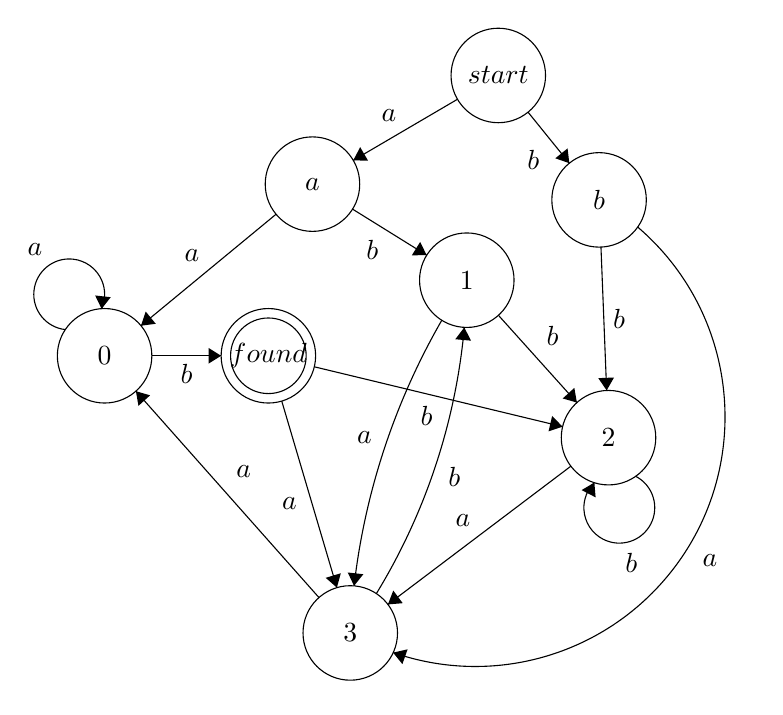
\begin{tikzpicture}[scale=0.2]
\tikzstyle{every node}+=[inner sep=0pt]
\draw [black] (11.3,-23.1) circle (3);
\draw (11.3,-23.1) node {$0$};
\draw [black] (34.3,-18.3) circle (3);
\draw (34.3,-18.3) node {$1$};
\draw [black] (43.3,-28.3) circle (3);
\draw (43.3,-28.3) node {$2$};
\draw [black] (26.9,-40.7) circle (3);
\draw (26.9,-40.7) node {$3$};
\draw [black] (21.7,-23.1) circle (3);
\draw (21.7,-23.1) node {$found$};
\draw [black] (21.7,-23.1) circle (2.4);
\draw [black] (36.3,-5.3) circle (3);
\draw (36.3,-5.3) node {$start$};
\draw [black] (24.5,-12.2) circle (3);
\draw (24.5,-12.2) node {$a$};
\draw [black] (42.7,-13.2) circle (3);
\draw (42.7,-13.2) node {$b$};
\draw [black] (33.71,-6.81) -- (27.09,-10.69);
\fill [black] (27.09,-10.69) -- (28.03,-10.71) -- (27.53,-9.85);
\draw (29.35,-8.25) node [above] {$a$};
\draw [black] (38.19,-7.63) -- (40.81,-10.87);
\fill [black] (40.81,-10.87) -- (40.7,-9.93) -- (39.92,-10.56);
\draw (38.94,-10.68) node [left] {$b$};
\draw [black] (22.19,-14.11) -- (13.61,-21.19);
\fill [black] (13.61,-21.19) -- (14.55,-21.07) -- (13.91,-20.29);
\draw (16.84,-17.16) node [above] {$a$};
\draw [black] (14.3,-23.1) -- (18.7,-23.1);
\fill [black] (18.7,-23.1) -- (17.9,-22.6) -- (17.9,-23.6);
\draw (16.5,-23.6) node [below] {$b$};
\draw [black] (8.816,-21.438) arc (263.94407:-24.05593:2.25);
\draw (6.88,-16.75) node [above] {$a$};
\fill [black] (11.11,-20.12) -- (11.69,-19.38) -- (10.7,-19.27);
\draw [black] (45.15,-14.924) arc (49.44438:-109.20303:15.858);
\fill [black] (29.62,-41.95) -- (30.21,-42.68) -- (30.54,-41.74);
\draw (49.24,-36.1) node [right] {$a$};
\draw [black] (42.82,-16.2) -- (43.18,-25.3);
\fill [black] (43.18,-25.3) -- (43.65,-24.48) -- (42.65,-24.52);
\draw (43.56,-20.74) node [right] {$b$};
\draw [black] (22.55,-25.98) -- (26.05,-37.82);
\fill [black] (26.05,-37.82) -- (26.3,-36.91) -- (25.34,-37.2);
\draw (23.53,-32.49) node [left] {$a$};
\draw [black] (24.62,-23.8) -- (40.38,-27.6);
\fill [black] (40.38,-27.6) -- (39.72,-26.92) -- (39.49,-27.9);
\draw (31.74,-26.28) node [below] {$b$};
\draw [black] (27.05,-13.79) -- (31.75,-16.71);
\fill [black] (31.75,-16.71) -- (31.34,-15.87) -- (30.81,-16.72);
\draw (28.3,-15.75) node [below] {$b$};
\draw [black] (36.31,-20.53) -- (41.29,-26.07);
\fill [black] (41.29,-26.07) -- (41.13,-25.14) -- (40.39,-25.81);
\draw (39.34,-21.84) node [right] {$b$};
\draw [black] (27.142,-37.71) arc (173.41001:150.02731:43.825);
\fill [black] (27.14,-37.71) -- (27.73,-36.97) -- (26.74,-36.86);
\draw (28.3,-28.3) node [left] {$a$};
\draw [black] (24.91,-38.45) -- (13.29,-25.35);
\fill [black] (13.29,-25.35) -- (13.45,-26.28) -- (14.19,-25.61);
\draw (19.64,-30.45) node [right] {$a$};
\draw [black] (34.144,-21.295) arc (-5.17826:-31.38442:39.268);
\fill [black] (34.14,-21.3) -- (33.57,-22.05) -- (34.57,-22.14);
\draw (33.09,-30.76) node [right] {$b$};
\draw [black] (40.91,-30.11) -- (29.29,-38.89);
\fill [black] (29.29,-38.89) -- (30.23,-38.81) -- (29.63,-38.01);
\draw (34.05,-34) node [above] {$a$};
\draw [black] (45.015,-30.747) arc (62.74616:-225.25384:2.25);
\draw (44.75,-35.58) node [below] {$b$};
\fill [black] (42.4,-31.15) -- (41.59,-31.63) -- (42.48,-32.09);
\end{tikzpicture}
\end{center}

Jak jsme poznamenali již dříve a je z obrázku vidět, že stavy \(1\) a \(2\) jsou v podstatě ekvivalentní a mohli bychom je sloučit
dohromady.  Ve skutečnosti lze ale celý automat ještě podstatně zjednodušit tak, aby
měl přesně o jeden stav více než je délka hledaného řetězce (\(m\)).  Stavy automatu
na obrázku odpovídají všem možným nejvýše dvouprvkovým posloupnostem písmen 
{\tt a,b}.  Například stav \(0\) odpovídá posloupnosti {\tt aa} zatímco třeba stav \(3\)
odpovídá posloupnosti {\tt ba}. Základní myšlenka spočívá v tom, že zahodíme všechny
stavy, které neodpovídají žádnému počátečnímu úseku hledaného řetězce.
Získáme tak automat znázorněný následujícím obrázkem:

\begin{center}
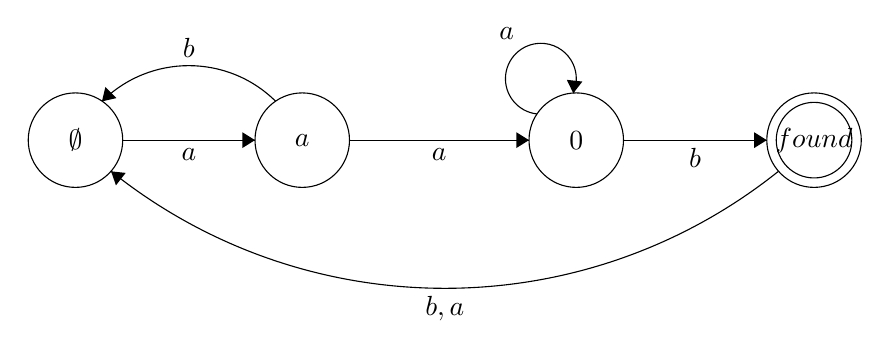
\begin{tikzpicture}[scale=0.2]
\tikzstyle{every node}+=[inner sep=0pt]
\draw [black] (42.6,-21.1) circle (3);
\draw (42.6,-21.1) node {$0$};
\draw [black] (57.7,-21.1) circle (3);
\draw (57.7,-21.1) node {$found$};
\draw [black] (57.7,-21.1) circle (2.4);
\draw [black] (10.8,-21.1) circle (3);
\draw (10.8,-21.1) node {$\emptyset$};
\draw [black] (25.2,-21.1) circle (3);
\draw (25.2,-21.1) node {$a$};
\draw [black] (28.2,-21.1) -- (39.6,-21.1);
\fill [black] (39.6,-21.1) -- (38.8,-20.6) -- (38.8,-21.6);
\draw (33.9,-21.6) node [below] {$a$};
\draw [black] (45.6,-21.1) -- (54.7,-21.1);
\fill [black] (54.7,-21.1) -- (53.9,-20.6) -- (53.9,-21.6);
\draw (50.15,-21.6) node [below] {$b$};
\draw [black] (40.116,-19.438) arc (263.94407:-24.05593:2.25);
\draw (38.18,-14.75) node [above] {$a$};
\fill [black] (42.41,-18.12) -- (42.99,-17.38) -- (42,-17.27);
\draw [black] (12.482,-18.638) arc (134.70674:45.29326:7.844);
\fill [black] (12.48,-18.64) -- (13.4,-18.43) -- (12.7,-17.72);
\draw (18,-15.87) node [above] {$b$};
\draw [black] (13.8,-21.1) -- (22.2,-21.1);
\fill [black] (22.2,-21.1) -- (21.4,-20.6) -- (21.4,-21.6);
\draw (18,-21.6) node [below] {$a$};
\draw [black] (55.443,-23.075) arc (-51.3352:-128.6648:33.922);
\fill [black] (13.06,-23.08) -- (13.37,-23.97) -- (13.99,-23.18);
\draw (34.25,-31.01) node [below] {$b,a$};
\end{tikzpicture}
\end{center}

Zbývá ještě ukázat, že takový automat umíme sestrojit v čase \(O(m)\).  Sestrojit stavy
a základní ``dopředné'' šipky spojující tyto stavy od nejkratšího k nejdelšímu je jednoduché.
Potřebujeme však ještě dodat šipky jdoucí ``zpět''.  Řekněme, že jsme  v nějakém stavu \(s\) 
který odpovídá řetězci {\tt r}. Abychom mohli správně dodat šipky jdoucí ``zpět'', potřebovali
bychom znát stav \(s^\prime\) odpovídající řetězci {\tt r[1:]} (každá šipka jdoucí zpět totiž bude 
odpovídat nějaké šipce ze stavu \(s^\prime\)). Není však problém si tento stav uložit v nějaké
pomocné proměnné a tuto proměnnou postupně aktualizovat.  Celý algoritmus v Pythonu
(včetně funkce find) lze nalézt na výpisu \ref{alg:optimalfind}.

\src[firstline=3]{optimalfind}{Vyhledávání pomocí konečných automatů}

\subsection{Regulární jazyky}

V předchozím odstavci jsme zavedli pojem konečného automatu a ukázali, jak lze konečné
automaty využít pro rychlé hledání v textu. Nicméně samotný pojem konečného automatu 
je zajímavý i teoreticky, protože se dá ukázat, že charakterizuje třídu regulárních jazyků. 

\begin{definition} Je-li \(\Sigma\) množina znaků (\emph{abeceda}), značíme \(\Sigma^*\) množinu všech
(konečných) posloupností prvků množiny \(Sigma\). Prvkům množiny \(\Sigma^*\) budeme říkat
\emph{slova}.  \emph{Jazykem} v abecedě \(\Sigma\) pak rozumíme libovolnou podmnožinu \(L\subseteq\Sigma^*\).
\end{definition}

\begin{definition}  Třída \emph{regulárních jazyků} nad abecedou \(\Sigma\) je nejmenší třída \(\mathcal L\) splňující:
\begin{itemize}
  \item[(i)] Prázdný jazyk je prvkem \(\mathcal L\),
 \item[(ii)] Pro každý znak \(a\in\Sigma\) je \(\{a\}\in\mathcal L\),
 \item[(iii)] Třída \(\mathcal L\) je uzavřená na sjednocení a konkatenaci (jsou-li \(A,B\in\mathcal L\), pak jejich konatenace,
                     značená \(A\cdot B\), je jazyk sestávající ze slov tvaru \(w_Aw_B\), kde \(w_A\in A\) a \(w_B\in B\)).
 \item[(iv)] Třída \(\mathcal L\) je uzavřená na Kleeneho hvězdičku (je-li \(A\in\mathcal L\), pak i jazyk \(A^*\) je prvkem
                     \(\mathcal L\), kde \(A^*\) je nejmenší nadmnožina \(A\) obsahující prázdnou množinu a uzavřená na konkatenaci).
\end{itemize}
\end{definition}

Tato definice vypadá velmi abstraktně. Nicméně je překvapivé, že má mnoho různých ekvivalentních reformulací.
Jedna možná definice využívá konečné automaty:

\begin{theorem} Jazyk \(L\) je \emph{regulární}, pokud existuje konečný automat \(A\) takový, že
\(L\) je množinou slov \(w\) takových, že existuje posloupnost stavů \(\overline{s}\), že \((w,\overline{s})\) je
výpočtem (viz \ref{def:vypocet}) automatu \(A\). 
\end{theorem}

Nabízí se otázka, zda je každý jazyk regulární.  Jednoduchým argumentem se můžeme přesvědčit, že nikoliv: všech jazyků
je totiž nespočetně (kontinuum), ale konečných automatů je jen spočetně (každý konečný automat je konečný objekt).
Není příliš těžké dokonce přímo sestrojit neregulární jazyk.

\begin{cviceni} Ukažte, že jazyk nad abecedou \(\Sigma=\{(,)\}\) sestávající ze správně uzávorkovaných výrazů, nemůže
být regulární.  (Hint: uvažte řetězec začínající \(n+1\)-otevřenými závorkami, kde \(n\) je počet stavů daného automatu.)
\end{cviceni}

\paragraph{Regulární výrazy}
Ukážeme si ještě jinou ekvivalentní definici regulárního jazyka, která je bližší původní definici a používá pojem regulárního výrazu. 
Tento pojem zavedl americký matematik \person{Kleene} a umožňuje velmi kompaktní popis regulárních jazyků. Každému regulárnímu
výrazu \(R\) odpovídá jazyk \(L(R)\) dle následující definice

\begin{definition} \emph{Regulární výraz} nad abecedou \(\Sigma\) je definován rekurzivně:
\begin{itemize}
 \item \(\emptyset, \varepsilon\) jsou regulární výrazy, \(L(\emptyset)=\emptyset, L(\varepsilon) = \{\emptyset\}\),  t.j. prázdný jazyk a jazyk sestávající z prázdného slova,
 \item každý znak \(a\in\Sigma\) je regulárním výrazem, \(L(a) = \{a\}\),
 \item je-li \(r\) regulární výraz, pak i \((r)\) je regulární výraz a \(L((r)) = L(r)\),
 \item jsou-li \(r,s\) dva regulární výrazy, pak \(r|s\) a \(rs\) je regulární výraz a \(L(r|s)=L(r)\cup L(s)\),\(L(rs)=L(r)\cdot L(s)\) (alternace a konkatenace)
 \item je-li \(r\) regulární výraz, pak \(r^*\) je regulární výraz a \(L(r^*) = L(r)^*\) (Kleeneho hvězdička).
\end{itemize}
\end{definition}

Aby se předešlo zbytečnému množství závorek je stanovena standardní priorita operací: Kleeneho  hvězdička má nejvyšší prioritu, pak konkatenace a
nakonec alternace. 

\begin{example} Je-li \(\Sigma=\{a,b,c\}\), pak \(r=ac^*(aa|bb)^*\) je regulární výraz popisující jazyk sestávající ze slov začínajících písmenem \(a\), pokračujících libovolným počtem znaků \(c\)
a pak libovolným počtem dvojic znaků \(aa\) nebo \(bb\).
\end{example}

Následující věta říká, že regulární výrazy přesně popisují regulární jazyky.

\begin{theorem} Jazyk \(L\) nad abecedou \(\Sigma\) je regulární právě když existuje regulární výraz \(r\) takový, že \(L=L(r)\).
\end{theorem}


\subsection{Aritmetické výrazy}

\paragraph{Stromová reprezentace}
\paragraph{Infixová notace}
\paragraph{Prefixová a postfixová notace}
\paragraph{Převádění mezi notacemi}
\paragraph{Vyhodnocování}

\ifx\ucebnice\undefined
\renewcommand{\refname}{\textbf{Literatura}}
\bibliographystyle{mujstyl}
\bibliography{ref}

\end{document}
\fi
